\documentclass[11pt]{article}
\usepackage[document]{ragged2e} % no indent line
\usepackage{amsmath} % math
\usepackage{hyperref} % url
\usepackage{mathtools} % norm
\DeclarePairedDelimiter{\norm}{\lVert}{\rVert}
\usepackage{listings} % show code

\title{TP de Calcul Numérique}
\author{Nicolas BOUTON}
\date{2020}

\begin{document}

\maketitle

\section{Exercice 1}

Developpement limité : 

\begin{equation*}
  \begin{split}
    T(x_i + h) & = T(x_i) + h \left(\frac{\delta T}{\delta x} \right)_i + h^2 \left(\frac{\delta^2 T}{\delta x^2} \right)_i + O(h^2) \\
    T(x_i - h) & = T(x_i) - h \left(\frac{\delta T}{\delta x} \right)_i + h^2 \left(\frac{\delta^2 T}{\delta x^2} \right)_i + O(h^2)
  \end{split}
\end{equation*}

On somme et on inverse le signe :

\begin{equation*}
  \begin{split}
    - T(x_i + h) + 2 T(x_i) - T(x_i - h) = - h^2 \left(\frac{\delta^2 T}{\delta x^2} \right)_i + O(h^2) \\
    \frac{- T(x_i + h) + 2 T(x_i) - T(x_i - h)}{h^2} = - \left(\frac{\delta^2 T}{\delta x^2} \right)_i
  \end{split}
\end{equation*}

Or on a :

\begin{equation*}
  - k \left( \frac{\delta^2 T}{\delta x^2} \right)_i = g_i, k > 0
\end{equation*}

On se permet de négligé k car c'est une constante dans nos prochain calcul :

\begin{equation*}
  \begin{split}
    - T(x_i + h) + 2 T(x_i) - T(x_i - h) = h^2 g_i
  \end{split}
\end{equation*}

On écrit le système d'équation : 

\begin{equation*}
  \begin{array}{ll}
    u_0 = T_0 & i = 0 \\
    - u_0 + 2 u_1 - u_2 = h^2 g_1 & i = 1\\
    ... & ... \\
    - u_{k-1} + 2 u_k - u_{k+1} = h^2 g_k & i = k\\
    ... & ... \\
    - u_{n-1} + 2 u_n - u_{n+1} = h^2 g_n & i = n\\
    u_n = T_n & i = n + 1 \\
  \end{array}
\end{equation*}

Avec les conditions aux bords on obtient :

\begin{equation*}
  \begin{array}{l}
    2 u_1 - u_2 = h^2 g_1 + T_0 \\
    - u_{n-1} + 2 u_n = h^2 g_n + T_n \\
  \end{array}
\end{equation*}

Donc on explicite le système linéaire $Au = g$ :

\begin{equation*}
  A = \left[
    \begin{array}{ccccccc}
      2 & -1 & 0 & - & - & - & 0 \\
      -1 & 2 & -1 & . &  &  & |  \\
      0 & -1 & . & . & . &  & |  \\
      | & . & . & . & . & . & |  \\
      | & & . & . & . & -1 & 0  \\
      | & & & . & -1 & 2 & -1  \\
      0 & - & - & - & 0 & -1 & 2 \\
    \end{array}
    \right]
\end{equation*}

\begin{equation*}
  u = \left[
    \begin{array}{c}
      T_1 \\
      | \\
      T_n \\
    \end{array}
    \right]
\end{equation*}

\begin{equation*}
  g = \left[
    \begin{array}{c}
      h^2 T_1 + T_0 \\
      h^2 T_2 \\
      | \\
      h^2 T_{n-1} \\
      h^2T_n + T_1\\
    \end{array}
    \right]
\end{equation*}

Comme il n'y a pas de source de chaleur, on a $\forall i \in [ 1, n
] : h^2 g_i = 0$

D'où $g = \left[
  \begin{array}{c}
    T_0 \\
    0 \\
    | \\
    0 \\
    T_1 \\
  \end{array}
  \right]$

Et la solution analytique qui se déguage est : 

$$ T(x) = T_0 + x (T_1 - T_0) $$

\section{Exercice 2}
\subsection{Arch}
\subsubsection{Bibliothèque}

Pour l'intallation des bibliothèque \textbf{cblas} et \textbf{lapacke}
:
\newline
\$ sudo pacman -S cblas lapacke

\subsubsection{Makefile}

Il faut modifier la ligne qui link les librairie en linkant la
bibliothèque \textbf{cblas}:

\# \\
\# -- librairies \\
LIBS=-llapacke -lcblas -lm \\

\section{Exercice 3}
\subsection{Question 1}

Les matrices pour utiliser \textbf{BLAS} et \textbf{LAPACK} en \textbf{C} sont allouées
et déclarées de la même manière que les tableaux en \textbf{C}. Mais elles
doivent être stockées dans l'un des formats suivant :

\begin{itemize}
\item stockage conventionnel en 2 dimension (ex: int tab[10][10])
\item stockage compact pour les matrices symétrique, hermitienne et
  triangulaire (stockage dans un tableau à 1 dimension des éléments
  de la matrice supérieur ou inférieur)
\item stockage bandes pour les matrices à bandes (cad que les
  diagonales autour de la diagonale principale contiennent la
  plupart des NNZ) (GB et GE)
\item utilisation de 2 ou 3 tableaux à 1 dimension pour stocker les
  matrices bidiagonale et tridiagonale respectivement
\end{itemize}

source : \url{http://performance.netlib.org/lapack/lug/node121}

\subsection{Question 2}

\begin{itemize}
\item Les constantes LAPACK\_ROW\_MAJOR et LAPACK\_COL\_MAJOR
  signifie la priorité ligne ou colonne respectivement de la
  représentation de la matrice.
\item Effectivement, cet argument sert si on utilise un stockage
  par priorité ligne ou colonne car il faut préciser si on a utilisé
  une priorité ligne ou colonne pour stocker la matrice pour pouvoir
  faire les bons calculs.
\end{itemize}

\subsection{Question 3}
   
La \textbf{leading dimension} permet de savoir qu'elle élément correspond
à la prochaine colonne ou la prochaine ligne suivant le stockage
colonne ou ligne respectivement.

\begin{itemize}
\item Si on choisis un stockage priorité ligne, alors la \textbf{leading dimension}
  correspond au nombre d'élément d'une ligne pour
  pouvoir accéder à la ligne suivante.
\item Si on choisis un stockage priorité colonne, alors la \textbf{leading dimension}
  correspond au nombre d'élément d'une colonne pour
  pouvoir accéder à la colonne suivante.
\end{itemize}

\subsection{Question 4}
\subsubsection{Résumé}

La fonction LAPACKE\_dgbsv permet de calculer le résultat d'un
système linéaire du type $A * X = B$, avec \textbf{X} l'inconnu, \textbf{A} une
matrice et \textbf{B} le second membre, où \textbf{X} et \textbf{B} peuvent être des
vecteurs ou des matrices.

\subsubsection{Argument}

Elle prend en argument la dimension de la matrice, le nombre du
sous-diagonnale ainsi que de sur-diagonnale, la leading dimension de
\textbf{A} et de \textbf{B}, le nombre de colonne de \textbf{B} ainsi
que tableau d'entier pour stoker les indices de permutation.

\subsubsection{Implémentation}

Cette fonction implémente une décomposition \textbf{LU} à pivot partiel et
la méthode de dessente et de remonté.

\subsubsection{Note importante}

Pour la factorisation \textbf{LU}, la fonction a besoin d'un vecteur de
travail ou il stockera les pivots. Suivant le stockage choisis on
rajoutera une ligne ou une colonne avant de stocker notre matrice
car le vecteur doit apparaître en premier.

\subsubsection{Sources}

\url{http://www.math.utah.edu/software/lapack/lapack-d/dgbsv.html}
   
\subsection{Question 5}
A titre comparatif nous prendrons une matrice de taille 10 x 10.

\subsubsection{Stockage priorité colonne}

\begin{equation*}
  \begin{array}{rrrr}
    0.000000 &	0.000000  &	2.000000 &	-1.000000	\\
    0.000000 &	-1.000000 &	2.000000 &	-1.000000	\\
    0.000000 &	-1.000000 &	2.000000 &	-1.000000	\\
    0.000000 &	-1.000000 &	2.000000 &	-1.000000	\\
    0.000000 &	-1.000000 &	2.000000 &	-1.000000	\\
    0.000000 &	-1.000000 &	2.000000 &	-1.000000	\\
    0.000000 &	-1.000000 &	2.000000 &	-1.000000	\\
    0.000000 &	-1.000000 &	2.000000 &	-1.000000	\\
    0.000000 &	-1.000000 &	2.000000 &	-1.000000	\\
    0.000000 &	-1.000000 &	2.000000 &	0.000000	\\
  \end{array}
\end{equation*}

\subsubsection{Stockage priorité ligne}

\begin{equation*}
  \begin{array}{rrrrrrrrrr}
    0.000 &	0.000 &	0.000 &	0.000 &
    0.000 &	0.000 &	0.000 &	0.000 &
    0.000 &	0.000 \\	
    0.000 &	-1.000 &	-1.000 &	-1.000 &
    -1.000 &	-1.000 &	-1.000 &	-1.000 &
    -1.000 &	-1.000 \\
    2.000 &	2.000 &	2.000 &	2.000 &
    2.000 &	2.000 &	2.000 &	2.000 &
    2.000 &	2.000 \\	
    -1.000 &	-1.000 &	-1.000 &	-1.000 &
    -1.000 &	-1.000 &	-1.000 &	-1.000 &
    -1.000 &	0.000 \\
  \end{array}
\end{equation*}

Pour que le tableau soit affichable nous avons dû enlever les 3
derniers 0 de la sortie, mais cela ne change pas le résultat.

\subsubsection{Remarques}

Nous pouvons apercevoir que nous avons le bon résultat, étant donné
que la première ligne qui réservé à \textbf{BlAS} pour son vecteur de
travail est constitué de zéro ainsi que le premier élément de la
diagonale supérieur et le dernier élément de le diagonale
inférieur.\newline

De plus pour vérifier le résultat il suffit de calculer la transposé
de l'une des matrices et la comparé à la deuxième car elles doivent
être égales. Ici la transposé d'une des 2 matrices est égales à la
deuxième.

\section{Exercice 5}

\subsection{Question 1}

\subsubsection{Equation}

La fonction \textbf{cblas\_dgbmv} permet de calculer l'équation
suivante :

\begin{equation*}
y = \alpha * A * x + \beta * y
\end{equation*}

Dans notre cas on a l'équation suivante :

\begin{equation*}
A * u = b
\end{equation*}

Qu'on peut écrire avec les notations de l'équation juste au dessus :

\begin{equation*}
A * y = x
\end{equation*}

Avec la question précédente on a calculer y. On peut donc tester la
fonction sur l'équation suivante :

\begin{equation*}
x = 1 * A * y + 0 * x
\end{equation*}

\subsubsection{Argument}

La fonction \textbf{cblas\_dgbmv} prends à peut près les mêmes
paramètres que \textbf{LAPACKE\_dgbsv} plus les coefficient $\alpha$
et $beta$, le nombre de ligne et de colonne de la matrice en format
classic ainsi qu'un paramètre qui indique si la matrice est une
transposé ou non.\newline

La fonction prend comme précondition que y et x soit des vecteurs.

\subsubsection{Note importante}

Contrairement à la fonction \textbf{LAPACKE\_dgbsv}, la fonction
\textbf{cblas\_dgbmv} n'attend pas à ce qu'on lui laisse un vecteur au
début de la matrice.

\subsection{Question 2}

Comme méthode de validation, nous proposons de calculé l'erreur
relative suivante.\newline

Etant donné que nous calculons l'équation suivante :

\begin{equation*}
b = A * u
\end{equation*}

Nous allons calculer l'erreur relative suivante :

\begin{equation*}
relres = \frac{\norm{b - A * u}}{\norm{b}}
\end{equation*}

Le résultat exacte de \textbf{B} est stocké dans le fichier \textbf{B.dat}.

\subsubsection{Priorité Ligne}

Le résultat est stocké dans le fichier \textbf{Y\_row.dat}.\newline

Cela ne marche pas encore.

\begin{lstlisting}
--------- Poisson 1D ---------


 INFO DGBSV = 0

The relative residual error is relres = 1.764638e-16

 DGBSV :

The relative residual error is relres = 5.102197e-16


--------- End -----------
\end{lstlisting}

Pour la priorité ligne il faut stocké les lignes en colonne et mettre
comme leading dimension la leading dimension des colonnes donc
conformément au code FORTRAN de BLAS qui stipule que la transposé de
la matrice est calculé et utilisé à la place de la matrice d'entré si
jamais on entre l'argument \textbf{CblasNoTrans}.

\subsubsection{Priorité Colonne}

Le résultat est stocké dans le fichier \textbf{Y\_col.dat}.

\begin{lstlisting}
--------- Poisson 1D ---------


 INFO DGBSV = 0

The relative residual error is relres = 1.764638e-16

 DGBSV :

The relative residual error is relres = 5.102197e-16


--------- End -----------
\end{lstlisting}

\subsubsection{Explication}

L'erreur relative de la fonction \textbf{cblas\_dgbmv} est un peut
plus élevé que l'erreur relative de la fonction
\textbf{LAPACKE\_dgbsv} qui peut être expliqué par le fait que le bit
de signe ne change pas et nous nous retrouvons avec des zéro négatif
au lieu de positif mais l'erreur reste acceptable car il est de
l'ordre de la précision machine.

\subsubsection{Conclusion}

Nous pouvons donc validé l'appelle a blas pour la priorité colonne
mais pas pour la priorité ligne pour le moment.

\section{Exercice 5}

\subsection{Question 1}

Le code scilab de la fonction se trouve dans le fichier
\textbf{src/facto\_lu.sci}.

\subsection{Question 2}

Le code scilab du script de test se trouve dans le fichier
\textbf{src/script\_facto\_lu.sci}.

\subsubsection{Graphiques}

\underline{Temps :}

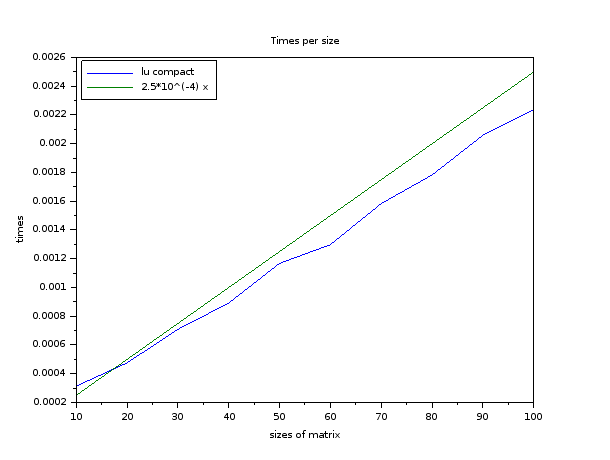
\includegraphics[scale=0.5]{img/lu_times.png}

\begin{itemize}
\item Nous pouvons apercevoir que le temps est plutôt linéaire.
\end{itemize}

\underline{Conditionnement :}

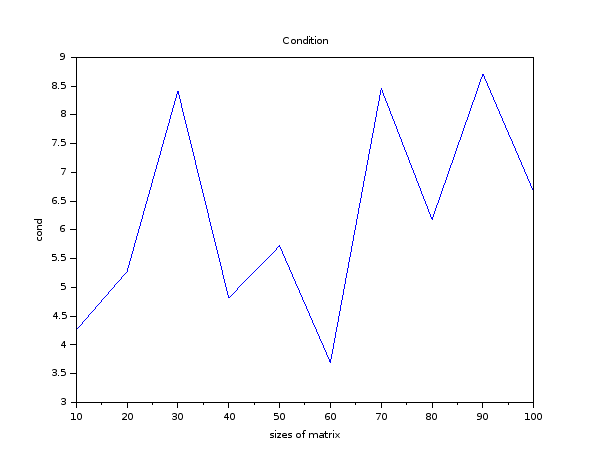
\includegraphics[scale=0.5]{img/lu_cond.png}

Le conditionnement reste bon pour des tailles de matrice entre 10 et
100 étant donné qu'il ne dépasse pas $10^{10}$, ce qui rendrait l'erreur
pour un double une erreur pour un float.\newline

\underline{Erreur relative avant :}

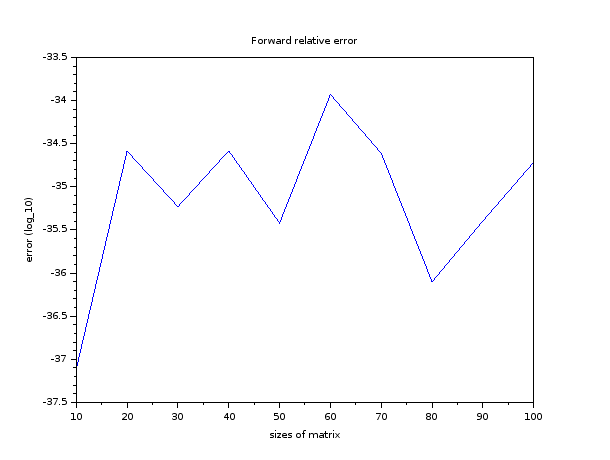
\includegraphics[scale=0.5]{img/lu_compact_error.png}

L'erreur relative arrière est respectable étant donné qu'elle est de
l'ordre de $10^{-34}$ pour des matrices de taille \textbf{100 x 100} ce
qui donne des bornes pour l'erreur vers $10^{-24}$ (étant donné
que le conditionnement est de $\approx 10^{10}$). Et cette
borne est également respectable comparé à la précision machine de
$10^{-16}$.

\subsubsection{Conclusion}

Donc nous pouvons dire que l'algorithme et son implémentation est
validé.

\section{Exercice 6}

\subsection{Question 1}

\subsection{Question 2}

\subsection{Question 3}

\subsection{Question 4}

\subsection{Question 5}

\section{Annexe}

Dépôt github : \url{https://github.com/Sholde/CN/tree/master/partie_2/poisson}

\end{document}
